\documentclass[10pt]{exam}
\usepackage[phy]{template-for-exam}
\usepackage{tikz}
\usepackage[top=0.2in, bottom=0.5in, left=1in, right=1in]{geometry}


\begin{document}
\pagestyle{empty}

\def\mytitle{Unit 03 Test: Projectiles}

\newcommand{\topmatter} {
  \vspace{2em}
  {\noindent \Large \bf Instructions:}

  \vspace{1em}

  \noindent {\bf Please do not open this test until told to do so!}

  \begin{itemize}
    \item Put your name on both this page \emph{and} the next page.
    \item Bubble in the number that is on your class notebook where it says ``ZipGrade ID''
    \item When instructed, tear off this first page
    \item Write your answers to the free-response questions directly on the packet.
    \item Bubble in your answers to the multiple-choice questions here.
    \item You may write anywhere on the packet.
    
  \end{itemize}

}
\newcommand{\bottommatter}{
%
}

\newcommand{\drawscantron}[2]{
  \begin{flushright}
    \begin{tikzpicture}
      \node[anchor=south west] at (0,0) {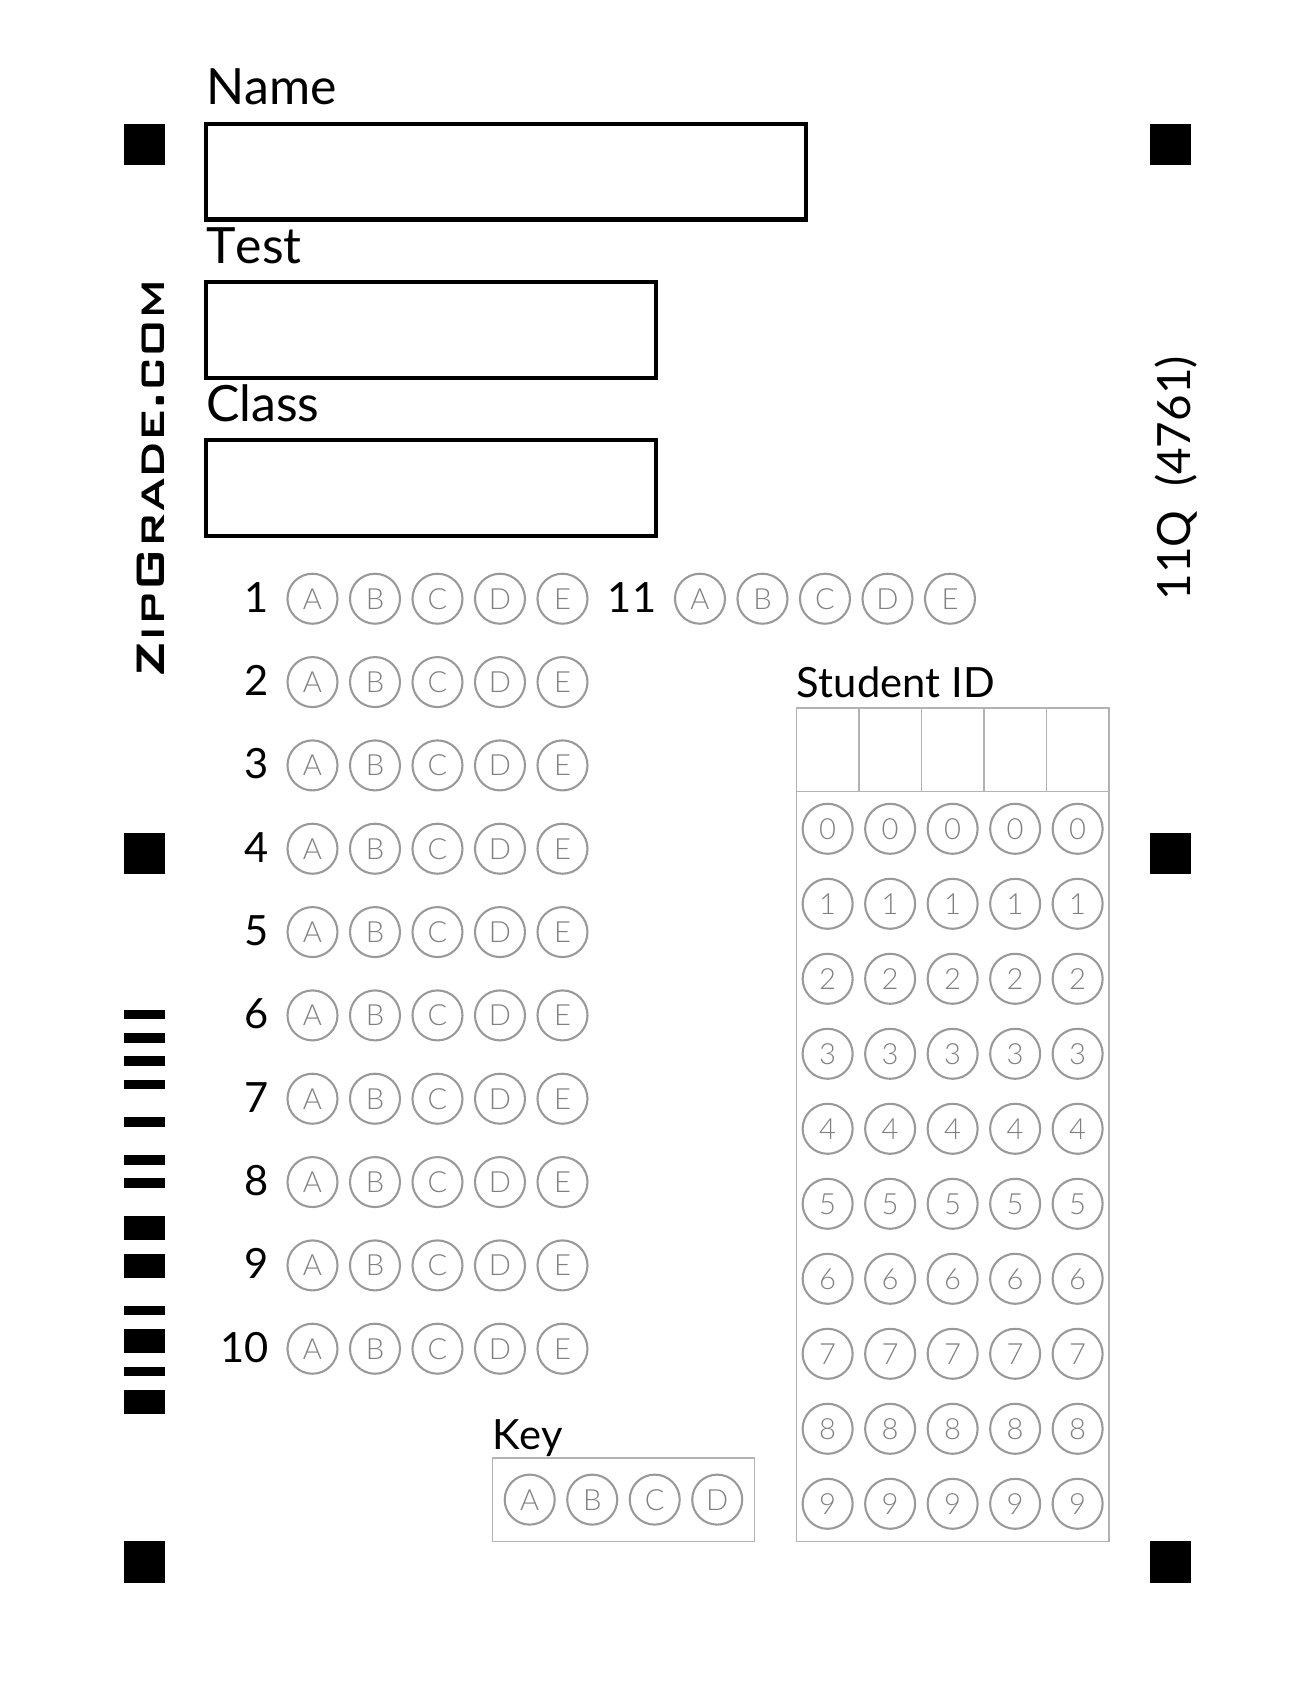
\includegraphics[width=.7\textwidth]{scantron.png}};
      \fill (#1,#2) circle (0.25);
      \node[anchor=west] at (2,12.25) {\small \mytitle};
      \fill[white] (7.1,8.8) rectangle (8.2,1.5);
      \node[fill=white] at (8.4,9.05) {\bf ZipGrade ID:};
    \end{tikzpicture}
  
    \bottommatter
  \end{flushright}
}



  \drawscantron{4.8}{1.9}
  \topmatter

\pagebreak

  \drawscantron{5.3}{1.9}
  \topmatter



\end{document}